%______________________________________________________________________________
% main.tex

\input{preamble12-screen.tex}
\hypersetup{%
    pdfauthor={Mike Pierce}%
   ,pdftitle={Math N16B Homework Two, Summer 2021}%
   ,pdfkeywords={Pierce,MathN16B,16B,N16B,Calculus,Integration,Berkeley}%
}
\usepackage{fourier}
\input{accessible-colors.tex}
\input{newcommand.tex}
\input{newenvironment.tex}
\pagestyle{empty}


\begin{document}

\begin{center}
    {\Huge{Homework Two}}
    \\ \footnotesize{Analytic Geometry and Calculus}
    \\ \footnotesize{UC Berkeley Math N16B, Summer 2021}
\end{center}
\vspace{2em}

Upload your responses to the prompts marked
(\textsc{\textcolor{magenta}{Submit}})
to Gradescope before 8pm Friday; 
you will receive feedback on these.
\begin{center}
    \href{https://www.gradescope.com/courses/275664}%
    {\texttt{gradescope.com/courses/275664}}
\end{center}
The rest of the exercises you should complete at your discretion.
Note that \emph{Calculus with Applications, 11th Edition} 
has some select solutions, usually to odd-numbered exercises, in the back.


\section*{Goals this Week}

Here are some goals you should have in mind while exercising:
\begin{enumerate}
    \item 
        Appreciate convergence.
        Whether or not an integral converges 
        should be answered with care
        since it's easy to get tripped up by $\infty$,
        but it's the question at the core 
        of some much more interesting and important questions. For example, 
        \emph{Does my algorithm finish or just run indefinitely?} or
        \emph{Does my mathematical model accurately describe this situation in the long-term?}
    \item 
        Gain some proficiency working with trigonometric integrands.
    \item 
        Learn when performing a trigonometric substitution will help you
        evaluate an integral. Generally just practice taking more integrals too,
        and appreciate how massively helpful making a substitution can be;
        changing variables has versatility beyond just letting $u$ 
        be the gross thing in an integrand.
\end{enumerate}
\newpage


\section*{Exercises}

\begin{enumerate}
    \item % IMPROPER INTEGRALS
        From Chapter 8.4 of \emph{Calculus with Applications, 11th Edition}
        work through the integration drills 
        at the beginning of the Exercises section,
        doing like every other odd integral.
        Also look at the following exercises:

        \begin{center}
            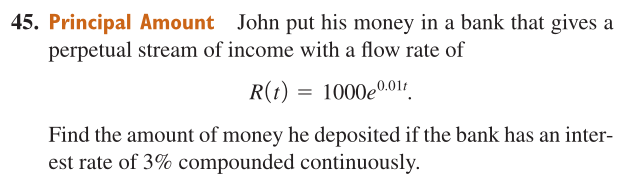
\includegraphics[width=\textwidth]{screenshots/45.png}
        \end{center}

        \begin{center}
            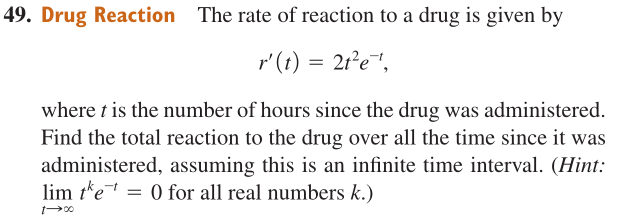
\includegraphics[width=\textwidth]{screenshots/49.png}
        \end{center}

    \item 
        (\textsc{\textcolor{magenta}{Submit}})
        Evaluate the integral 
        \begin{equation*}
            %% This is same as one in teh next exercise ...
            \int\limits_2^\infty \frac{\dx}{x\left(\ln(x)\right)^2}
            \,.
        \end{equation*}

    \item 
        (\textsc{Improper Integrals})
		In case you'd like \emph{even more} practice, 
        evaluate each of the following integrals.
        Some of these I borrowed from 
        \href{http://tutorial.math.lamar.edu/Problems/CalcII/ImproperIntegrals.aspx}%
        {Paul's Online Math Notes},
        so you might find solutions there. 
        \begin{tasks}[after-item-skip=2ex](3)
            \task $\displaystyle\int_{0}^{\infty} x\ex^{-x} \dx$
            \task $\displaystyle\int_{\ex}^{\infty} \frac{\dx}{x\ln(x)^2}$
            \task $\displaystyle\int_{0}^{\pi/2} \frac{\cos(x)}{\sqrt{\sin(x)}} \dx$
            \task $\displaystyle\int_{-5}^{1} \frac{1}{10+2z} \dz$
            \task $\displaystyle\int_{0}^{4} \frac{x}{x^2-9} \dx$
            \task $\displaystyle\int_{-\infty}^{\infty} \frac{6w^3}{(w^4+1)^2} \dw$
            \task $\displaystyle\int_{-1}^{1} \ln|x| \dx$
            \task $\displaystyle\int_{1}^{\infty} \frac{1}{x^3} \dx$
            \task $\displaystyle\int_{1}^{\infty} \frac{1}{x^{1/3}} \dx$
            \task $\displaystyle\int_{-\infty}^{1} \frac{3}{1+x^2} \dx$
            \task $\displaystyle\int_{-\infty}^{0} \frac{\ex^{\frac{1}{x}}}{x^2} \dx$
            \task $\displaystyle\int_{0}^{2} \frac{1}{(x-1)^4} \dx$
        \end{tasks}

	\item
        Let's define the function $A(z) = \int_1^z x^{-p} \dx$
        for $z>1$.
        \begin{enumerate}
        \item Show that if $p=1$, then $A(z) = \ln|z|$,
              but that otherwise, for $p\neq 1$, we have 
              \begin{equation*}
                  A(z) = \frac{1}{1-p}\left(z^{1-p}-1\right)\,.
              \end{equation*}
            \vspace{-6ex}
        \item Show that if $p \in (0,1]$,
            then $\lim_{z \to \infty} A(z) = \infty$.
        \item Now show that if $p > 1$,
            then $\lim_{z \to \infty} A(z) = \frac{1}{p-1}$.
        \end{enumerate}
		Look out for the vocabulary term \term{$p$-series} 
		later in the course, and remember this exercise when you see it ;)

    \item 
        (\textsc{Challenge, Spivak})
        Consider the curve given by $y = \frac{1}{x}$ for $x \geq 1$.
        This shape is sometimes called 
        \href{https://en.wikipedia.org/wiki/Gabriel's_Horn}{Gabriel's horn}.
        \begin{enumerate}
        \item What is the volume of the inside of the horn?
        \item You can find the surface area of the horn 
            by taking the curve $y = \frac{1}{x}$,
            writing down a formula for it's arclength, 
            and rotating that arclength about the $x$-axis
            over a bunch of small subintervals,
            and taking an integral, 
            thereby summing up a lot of smaller surface areas.
            Do this, and show that the horn has infinite surface area.
        \item Suppose you take a volume of paint that is equal to 
            the volume of the inside of the horn and pour it into the horn.
            This would seem to paint the entire inside of the horn,
            but we will have painted the infinite surface of the horn
            with finitely much paint. How can this be?
        \end{enumerate}

    \item % Derivatives of trig functions
        Review Chapter 13.2 of \emph{Calculus with Applications, 11th Edition}
        and make sure you remember the trig functions
        and their derivatives.

    \item % Integrals involving trig functions
        From Chapter 13.3 of \emph{Calculus with Applications, 11th Edition}
        work through the integration drills 
        at the beginning of the Exercises section,
        doing like every other odd integral.
        Also look at the following exercises:
        \begin{center}
            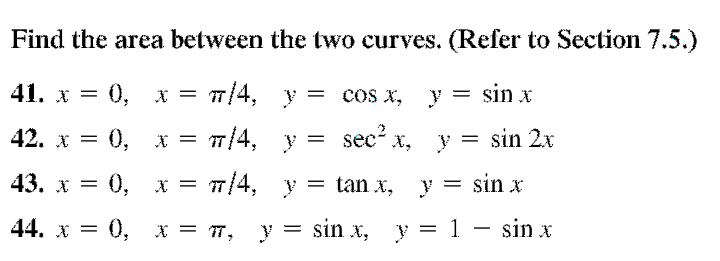
\includegraphics[width=\textwidth]{screenshots/41.png}
        \end{center}
        \begin{center}
            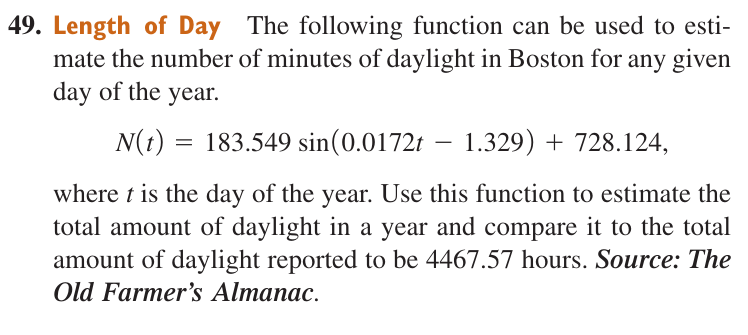
\includegraphics[width=\textwidth]{screenshots/49again.png}
        \end{center}

    \item 
        (\textsc{Trigonometric Integrals})
        Evaluate \emph{some} of the following integrals for practice.
        These are a bit tougher than the ones in the textbook.
        Solutions to a couple of them can be found in 
        \href{http://tutorial.math.lamar.edu/Problems/CalcII/IntegralsWithTrig.aspx}%
        {Paul's Online Notes}.
        \begin{tasks}[after-item-skip=2ex](2)
            %
            \task $\displaystyle\int \sin^2(x)\cos^7(x)\dx$
            % TOO HARD, try different powers of sec and tan
            %\task $\displaystyle\int \sec^3(x)\tan^4(x)\dx$
            %
            \task $\displaystyle\int \cos^4(\theta) \dtheta$
            %
            \task $\displaystyle\int \tan^3(\mu)\dmu$ 
            (\textsc{\textcolor{magenta}{Submit}})
            %
            \task $\displaystyle\int \cot(10z)\csc^4(10z)$
            %
            %\task $\displaystyle\int \frac{2+7\sin^3(x)}{\cos^2(x)}\dx$
        \end{tasks}

    \item 
        (\textsc{Trigonometric Substitution})
        Evaluate \emph{some} of the following integrals.
        They all require the same trick of making a trigonometric substitution,
        so only do as many as it takes you to feel good. 
        \begin{tasks}[after-item-skip=2ex](3)
            %
            \task $\displaystyle\int \frac{\dx}{1+x^2}$
            %
            \task $\displaystyle\int \frac{\dx}{1-x^2}$
            %
            \task $\displaystyle\int \frac{\dx}{\sqrt{1-x^2}}$
            %
            \task $\displaystyle\int \frac{\dx}{\sqrt{1+x^2}}$
            % becomes \int\sec(x)\dx, then needs tan(arcsec(x))
            \task $\displaystyle\int \frac{\dx}{\sqrt{x^2-1}}$
            % So chill it's just arcsec(x)
            \task $\displaystyle\int \frac{\dx}{x\sqrt{x^2-1}}$
            (\textsc{\textcolor{magenta}{Submit}})
            %
            \task $\displaystyle\int \frac{\dx}{x\sqrt{1-x^2}}$
            %
            \task $\displaystyle\int \frac{\dx}{x\sqrt{1+x^2}}$
            %
            \task $\displaystyle\int x^3\sqrt{1-x^2}\dx$
            % becomes \int\cos^2(x)\dx, which requires half/double angles
            \task $\displaystyle\int \sqrt{1-x^2}\dx$ 
            %
            \task $\displaystyle\int \sqrt{1+x^2}\dx$
            %
            \task $\displaystyle\int \sqrt{x^2-1}\dx$
        \end{tasks}

    \item 
        (\textsc{Trigonometric Substitution})
        Here's some tougher integrals requiring trig substitution. 
        Evaluate them if you'd like to practice. 
        Solutions to these are written up in
        \href{http://tutorial.math.lamar.edu/Problems/CalcII/TrigSubstitutions.aspx}%
        {Paul's Online Math Notes}.
        \begin{tasks}[after-item-skip=2ex](3)
            \task $\displaystyle\int \sqrt{1-7\omega^2} \domega$
            \task $\displaystyle\int\limits_{-7}^{-5} \frac{2\dy}{y^4\sqrt{y^2-25}}$
            \task $\displaystyle\int \frac{\dx}{\sqrt{9x^2-36x+37}} $
        \end{tasks}

    \item 
        (\textsc{Tough})
        Evaluate the following integrals if you'd like.
        \begin{tasks}(3)
            \task $\displaystyle\int\limits \frac{\dx}{\sqrt{1+\ex^{2x}}}$
            \task $\displaystyle\int\limits \ln\left(\mu + \sqrt{1-\mu}\right)\dmu$
            \task $\displaystyle\int\limits \frac{\dtheta}{1-\sin^4(\theta)}$
        \end{tasks}

\end{enumerate}

\vspace{1em}
Since you've learned \emph{integration-by-parts},
and how to handle integrals with trigonometric functions,
and when you should make a substitution for a trig function,
you've officially learned all the techniques of integration 
that are in the curriculum for this course.
Congratulations! 
The exercises that follow are 
some integration-themed challenges,
in case you enjoy the puzzle of solving integrals like I do.

\begin{enumerate}[resume]
    \item (\textsc{Challenge: The $x \leftrightarrow \frac{1}{x}$ Trick})
        Show that the integral 
        \begin{equation*}
            \int\limits_{0}^{\infty} \frac{\ln(x)}{1+x^2} \dx
        \end{equation*}
        evaluates to zero by breaking up its domain of integration into two parts
        based on where the integrand is negative or positive,
        and using the substitution $x \leftrightarrow \frac{1}{x}$
        on one of those parts.
        Then use this same trick to show that the value of the following 
        integral doesn't depend at all on the value of the real number $a$.
        \begin{equation*}
            \int\limits_{0}^{\pi/2} \frac{\dtheta}{1+\big(\tan(\theta)\big)^a}
        \end{equation*}
        For some helpful reading related to this trick, see
        \begin{center}
            \href{https://math.stackexchange.com/q/2060187/167197}%
            {\texttt{math.stackexchange.com/q/2060187}}.
        \end{center}

    \item 
        (\textsc{Challenge})
        Evaluate the following integrals.
        \begin{tasks}(3)
            \task $\displaystyle\int\limits \frac{\domega}%
                {\left(\omega^2+1\right)\sqrt{\omega^2-1}} $
            \task $\displaystyle\int\limits \sqrt{\tan\left(\theta\right)} \dtheta $
            \task $\displaystyle\int\limits_{0}^{\pi/2} \ln\left(\cos(t)\right) \dt$
        \end{tasks}

    \item (\textsc{Challenge: 2005 Putnam Exam}) Evaluate
        \begin{equation*}
            \int\limits_0^1 \frac{\ln(x+1)}{1+x^2} \dx
            \,.
        \end{equation*}

    \item (\textsc{Challenge: 1987 Putnam Exam}) Evaluate
        \begin{equation*}
            % First thought is to take u=x+3 to center everything at x=0
            \int\limits_2^4 \frac{\sqrt{\ln(9-x)}}%
                {\sqrt{\ln(9-x)}+\sqrt{\ln(x+3)}} \dx
            \,.
        \end{equation*}

\end{enumerate}

You might also be interested in reading up on 
some lesser known integration tricks:
\begin{center}
	\href{http://math.stackexchange.com/q/70974/167197}%
	{\texttt{math.stackexchange.com/q/70974/167197}}.
\end{center}

\end{document}

